\section{Summary}

\begin{wideslide}[toc=Neutrino interactions]{Neutrino-nucleus interactions}
\null\vfill

  \sep

  For all channels (but coherent) neutrino interactions are factorized in the following way
  
  \sep\sep\sep
  
  \centering\input{figures/factorization}
  
  \sep\sep
  
  \begin{itemize}
   \item Is the physics really factorized this way?
   \item This factorization is common for all generators
   \item However, some pieces are done in different way
  \end{itemize}
  
\vfill\null
\end{wideslide}

\begin{slide}[toc=MiniBooNE CC $\pi$]{MiniBooNE data for CC $\pi$ production}

  \rput(12, 4.25)
  {
  \begin{pspicture}
   
    \pscircle[linestyle = none, fillstyle = solid, fillcolor = pdcolor1](0,0){1}

    \pscircle[linestyle = none, fillstyle = solid, fillcolor = pdcolor4](-2.5,0){0.2}
    \psline[linewidth = 0.05, linecolor = pdcolor4]{->}(-2.1,0)(-1.2,0)
    \rput[c](-1.75,0.25){\color{pdcolor4}\small $\left<E_\nu\right>$}
    \rput[c](-1.75,-0.24){\color{pdcolor4}\small $\sim 1$~GeV}
    \psline[linewidth = 0.05, linecolor = pdcolor1]{->}(1.2,0)(1.6,0)
    
    \rput[l](2,0.75){\color{pdcolor1} 1$\mu$}
    \rput[l](2,0){\color{pdcolor1} 0$\pi^\pm$ (0$\pi^{\overset{0}{-}}$)}
    \rput[l](2,-0.75){\color{pdcolor1} 1$\pi^0$ (1$\pi^+$)}
    
  \end{pspicture}
  }

  \begin{itemize}
   
   \item The cross section \\ for $\pi^0$ ($\pi^+$) production \\ through charge current \\ measured by MiniBooNE
   
   \item The signal is defined as: charged leptons, no charged pions and one neutral pion (one positive pion and no other pions) in the final state.
   
   \item The result depends on primary vertex and FSI, as pion can be:
   
   \vspace{5pt}
   
    \begin{itemize}
    
      \item produced in primary vertex
      \item produced in FSI
      \item affected by charge exchange
      \item absorbed
    
    \end{itemize}
    
  \end{itemize}
  
\end{slide}

\begin{wideslide}[toc=]{MiniBooNE data for CC $\pi$ production}
\null\vfill

  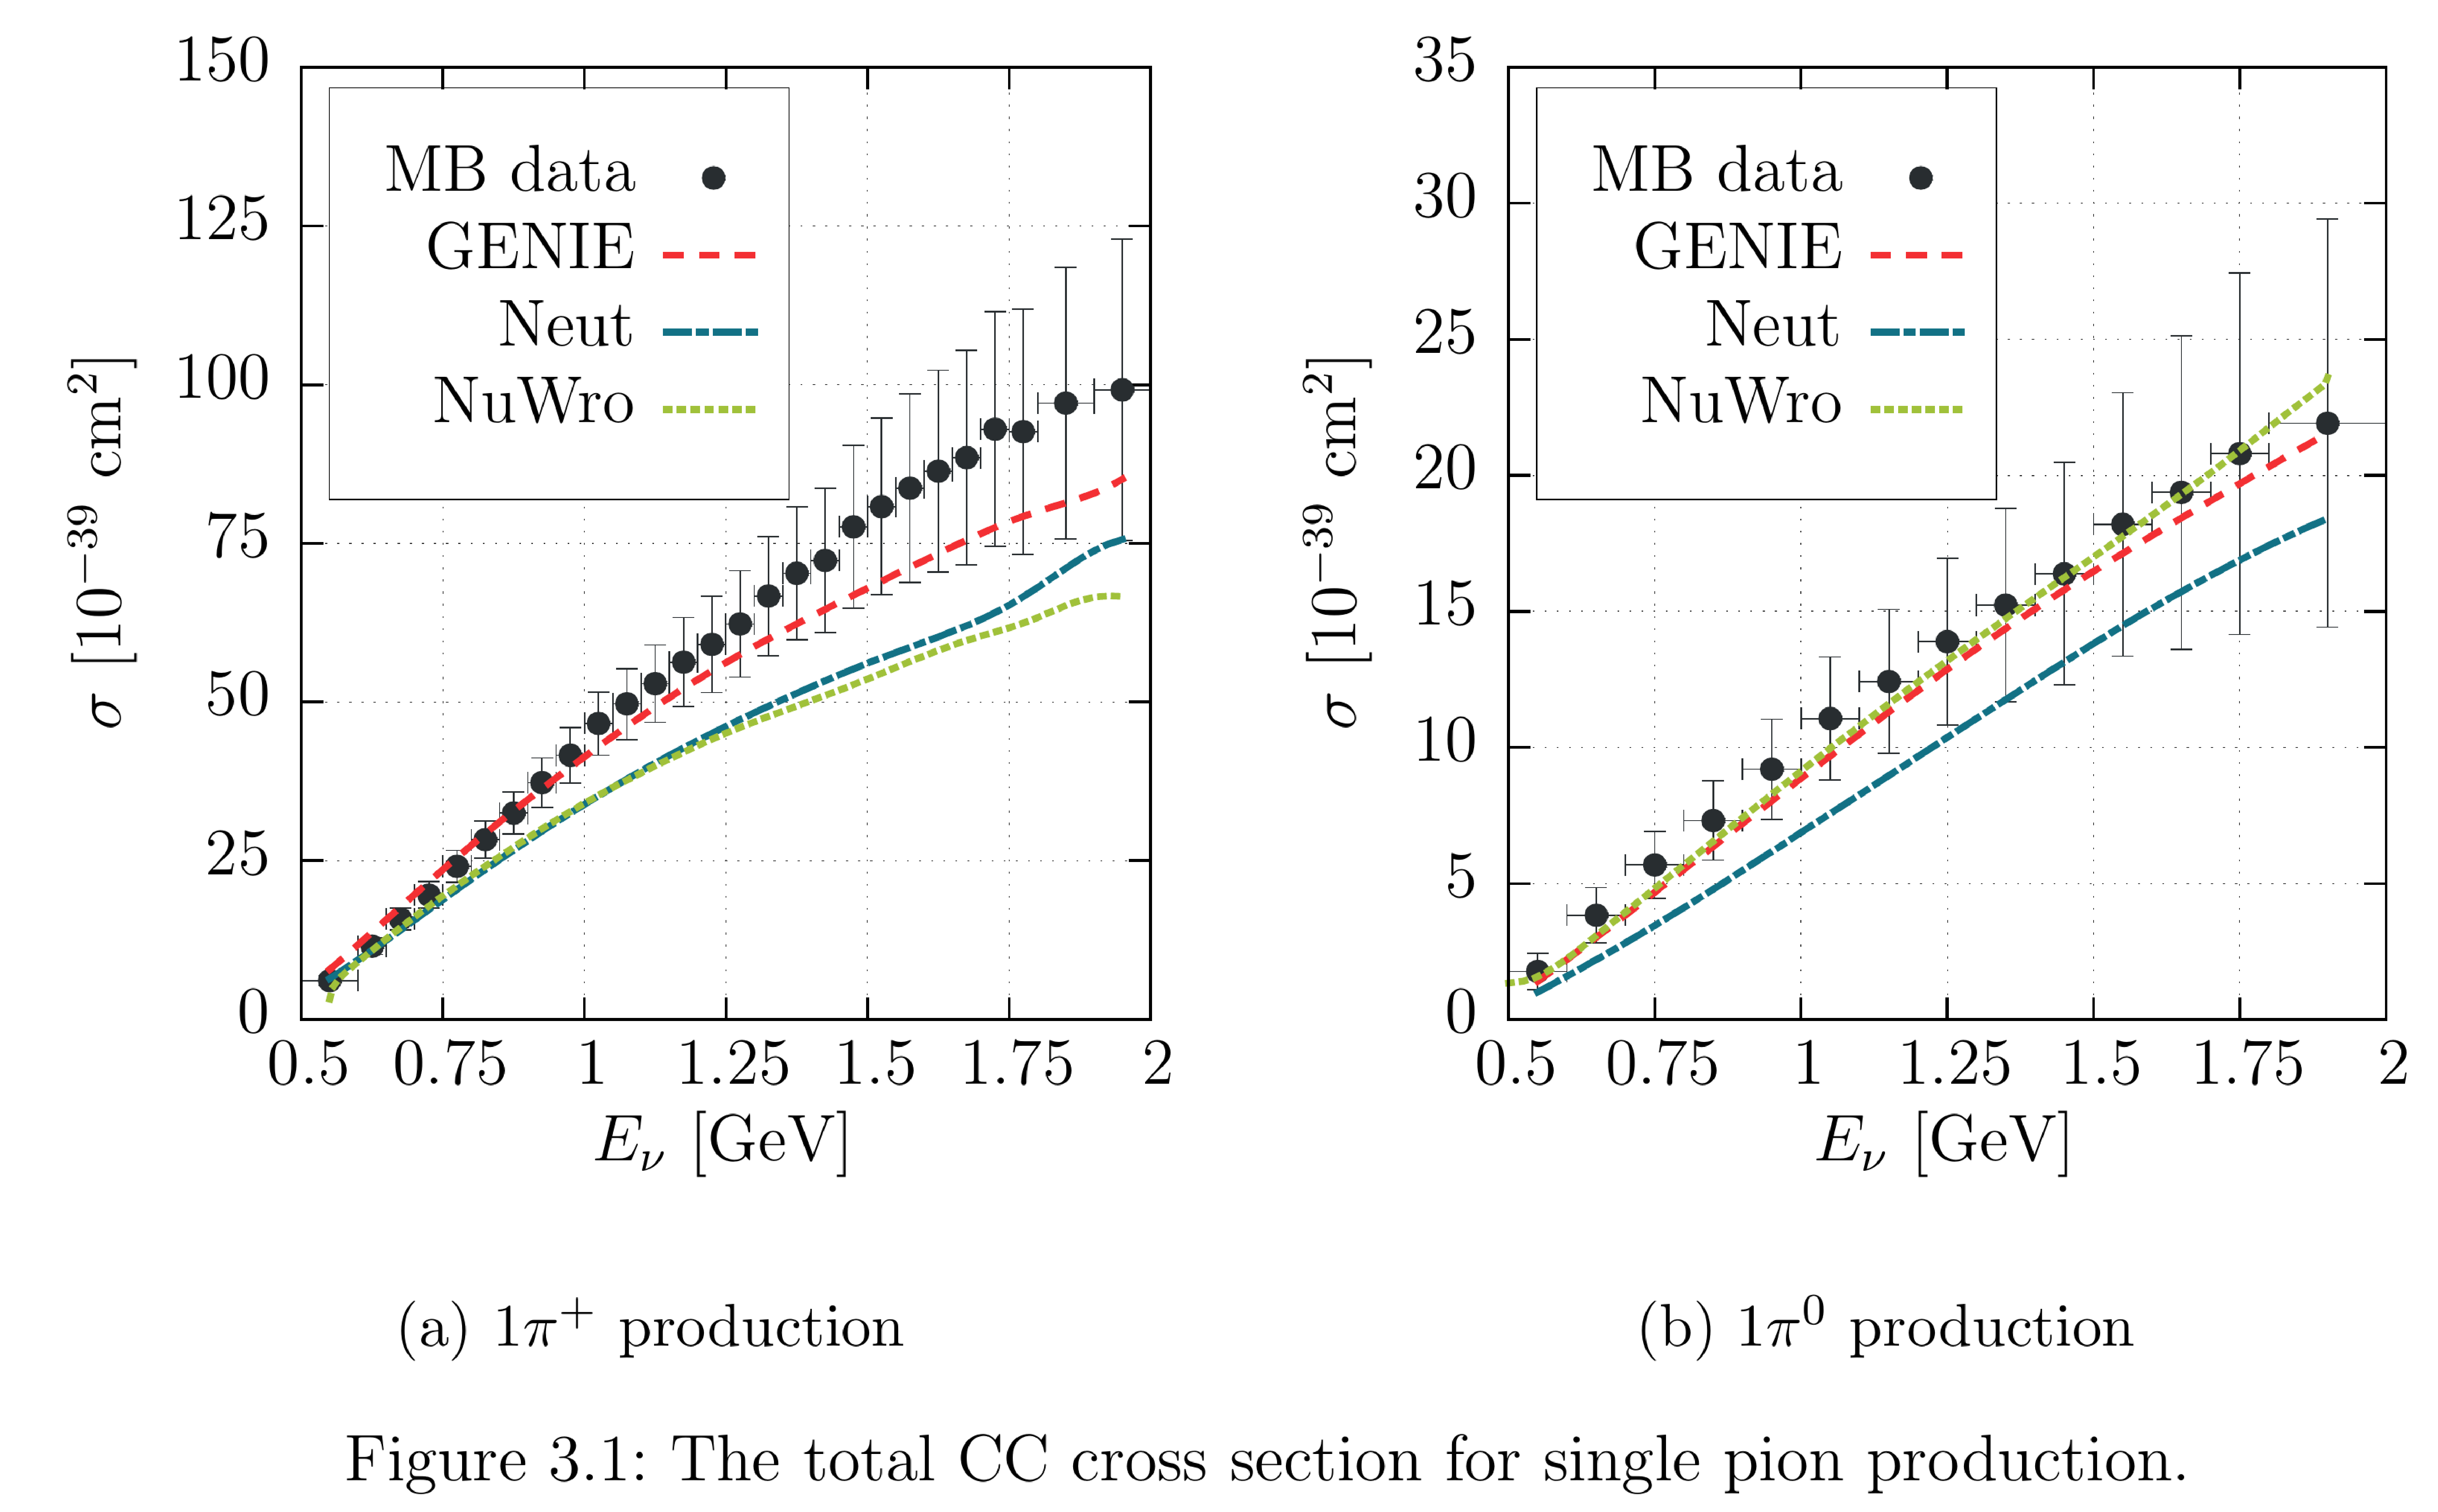
\includegraphics[width=\columnwidth]{figures/mbtot.eps}

\vfill\null
\end{wideslide}

\begin{wideslide}[toc=]{MiniBooNE data for CC $\pi$ production}
\null\vfill

  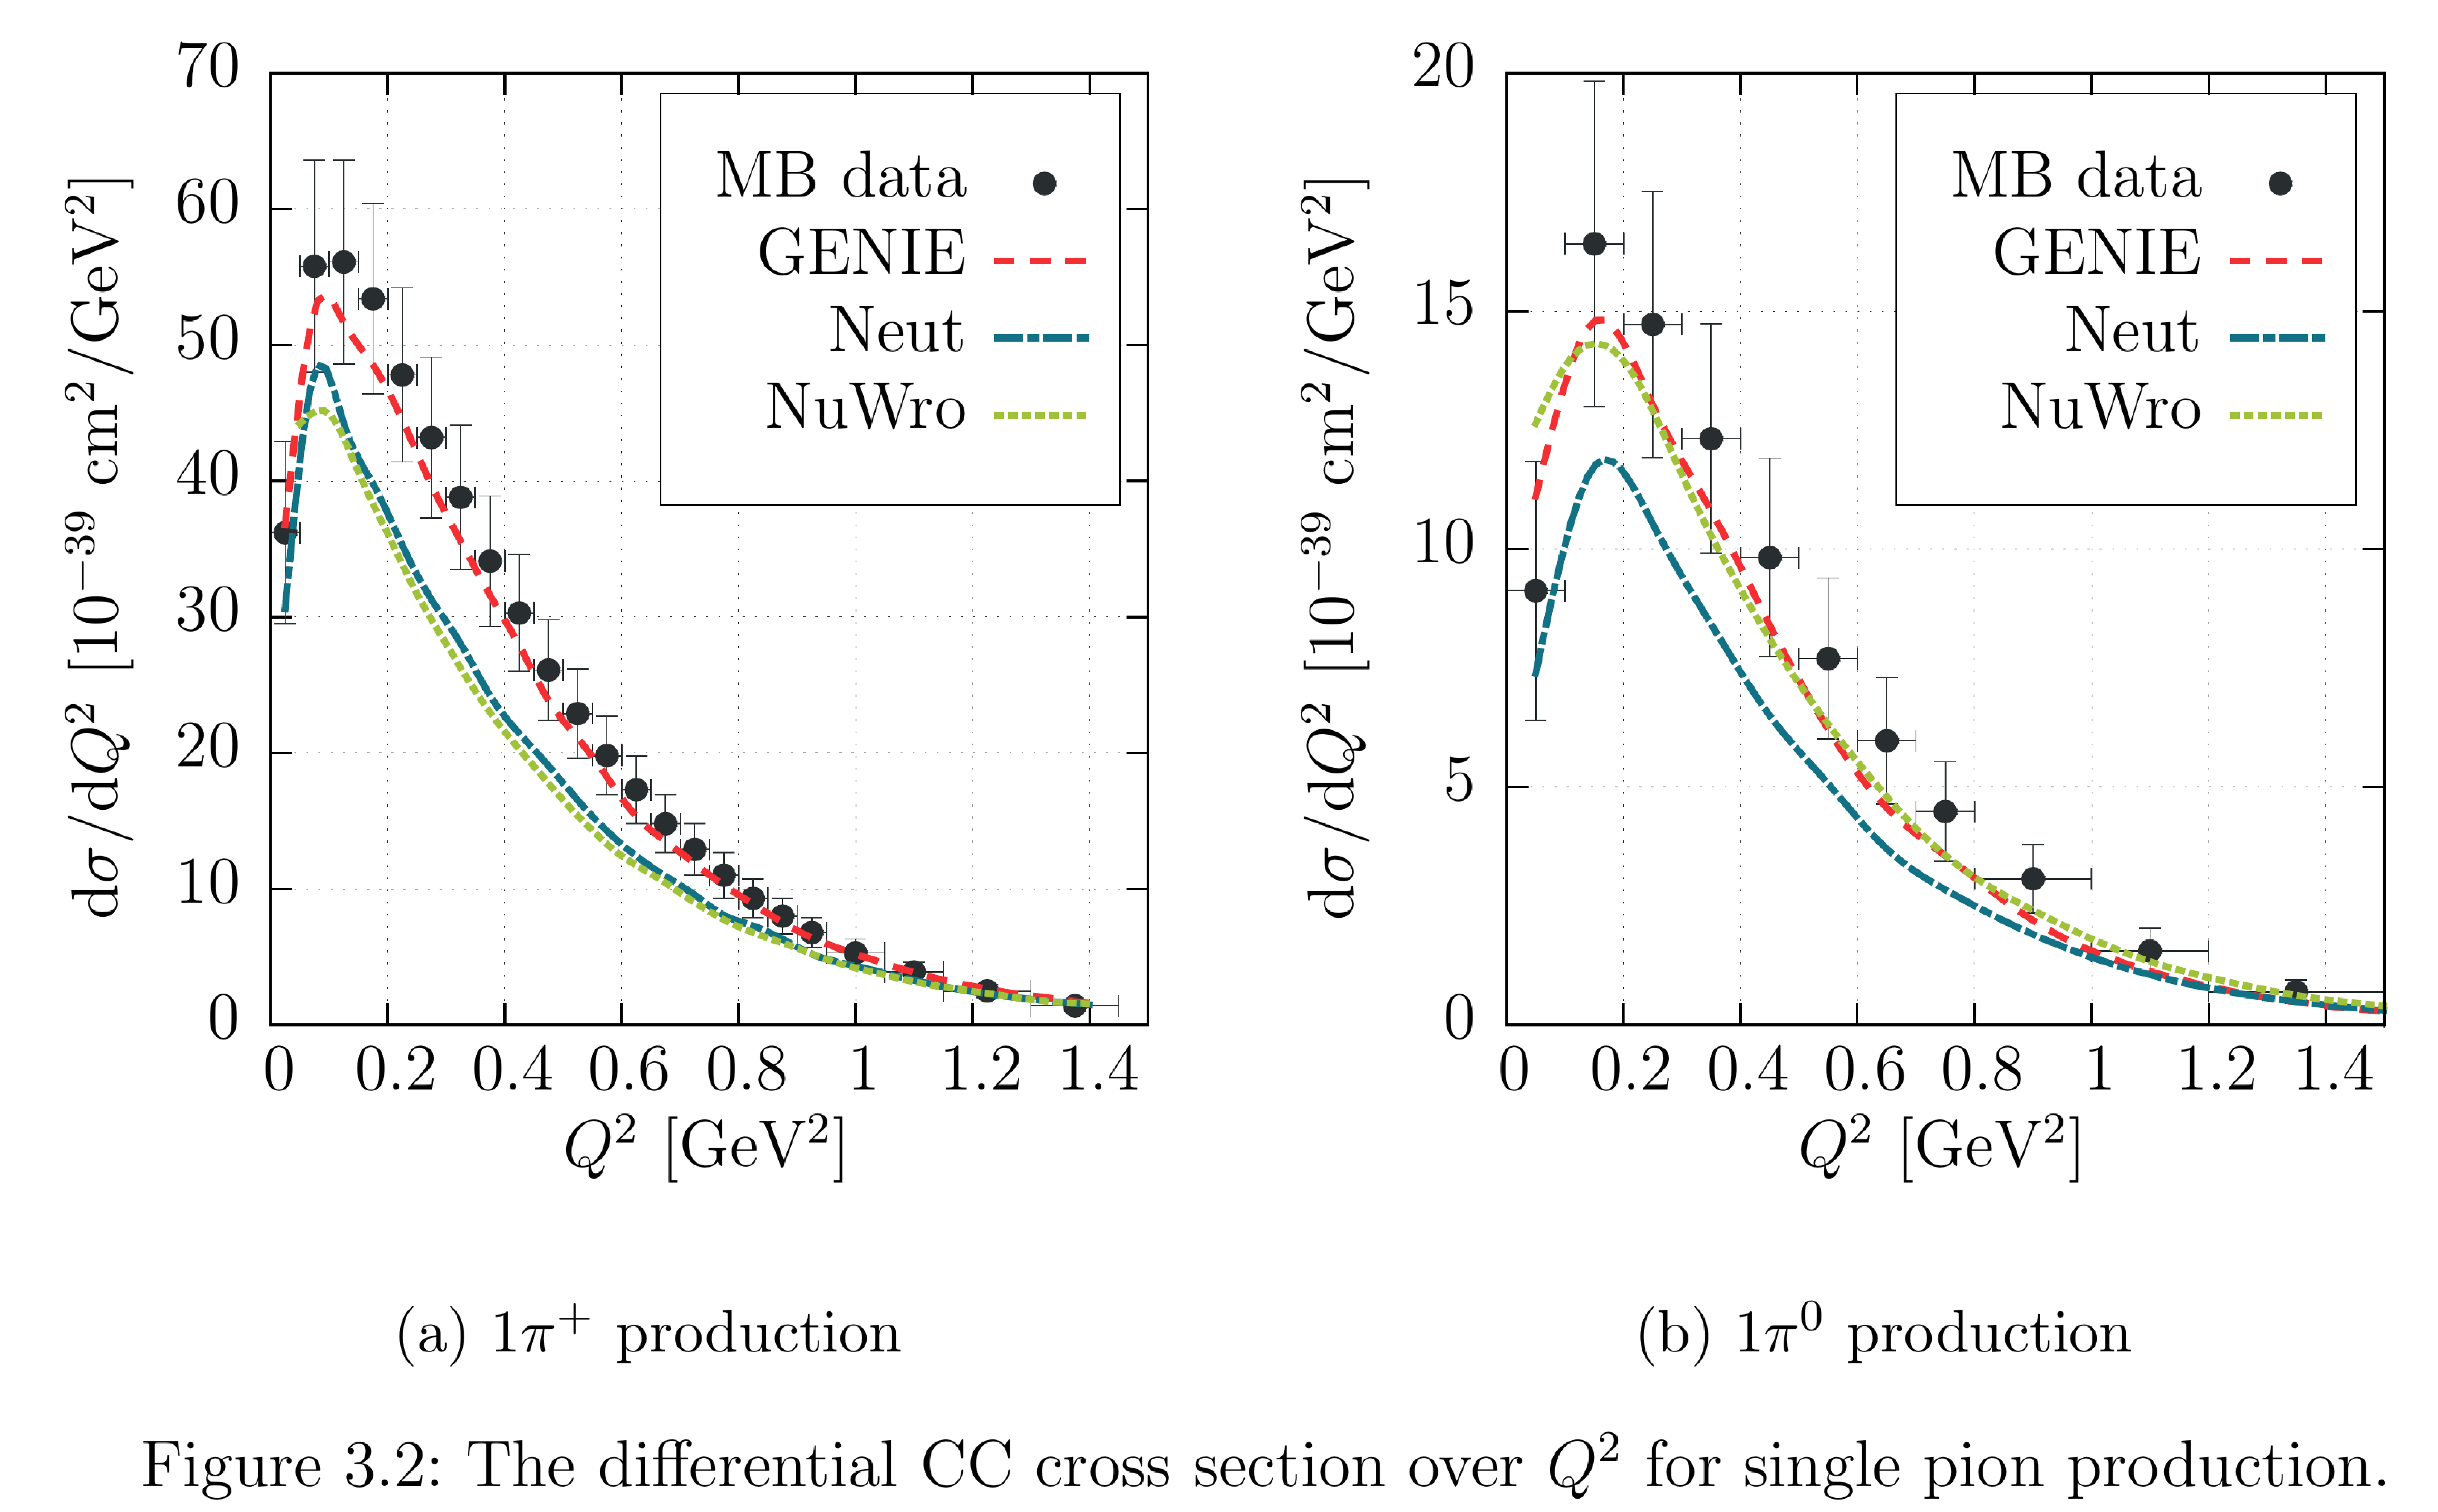
\includegraphics[width=\columnwidth]{figures/mbq2.eps}

\vfill\null
\end{wideslide}

\begin{slide}{Summary}
\null\vfill

  \rput(1.1\slidewidth, 0.55\slideheight){\scalebox{1.5}{\input{figures/mcgenlogo}}}

  \begin{itemize}
   \item MC generators are irreplaceable \\ tools in high-energy physics
   \item People use them before \\ experiment exists \\ (feasibility studies, requirements ...)
   \item And during data analysis \\ (systematics uncertainties, backgrounds ...)
   \item There are several neutrino event generators and they all differ slightly
   \item And, unfortunately, there is no one right generator
  \end{itemize}
  
\vfill\null
\end{slide}